\chapter{INPUT OPTICS DESIGN AND CHARACTERIZATION}

\section{Function of the Input Optics}
\label{sec:role}

\begin{figure}
\begin{centering}
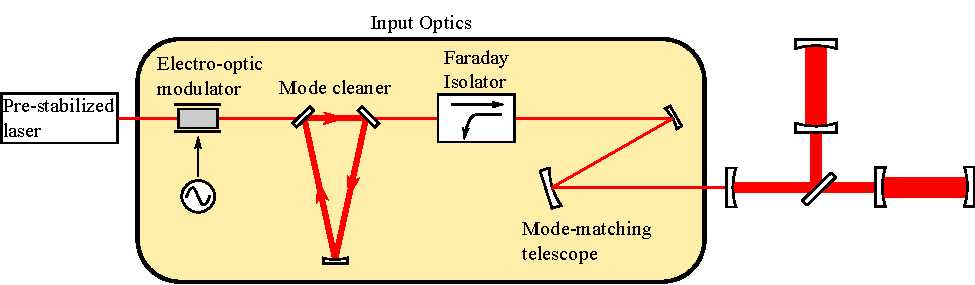
\includegraphics{figures/InputOpticsBlock_thesis.pdf}
\caption[Block diagram of the Input Optics subsystem.]{Block diagram
  of the Input Optics subsystem. The IO is located between the
  pre-stabilized laser and the recycling mirror and consists of four
  components: electro-optic modulator, mode cleaner, Faraday isolator,
  and mode-matching telescope. The electro-optic modulator is the only
  IO component outside of the vacuum system. Diagram is not to scale.}
\label{fig:IOblock}
\end{centering}
\end{figure}

The Input Optics (IO)\footnote{The Input Optics was originally called
  the Input-Output Optics (IOO).} is one of the primary subsystems of
the Laser Interferometer Gravitational-wave Observatory (LIGO)
interferometers. Its purpose is to deliver an aligned, spatially
pure, mode-matched beam with phase-modulation sidebands to the
power-recycled Fabry-Perot Michelson interferometer. The IO also
prevents reflected or backscattered light from reaching the laser and
distributes the control sidebands reflected from the interferometer
(designated the \emph{reflected port}) to photodiodes for sensing and
controlling the length and alignment of the interferometer. In
addition, the IO provides an intermediate level of frequency
stabilization and must have high overall optical efficiency. It must
perform these functions without limiting the strain sensitivity of the
LIGO interferometer.  Finally, it must operate robustly and
continuously over years of operation. The conceptual design is found
in Ref.~\citep{Camp1996InputOutput}.

As shown in Figure~\ref{fig:IOblock}, the Input Optics subsystem
consists of four principle components located between the
pre-stabilized laser and the power recycling mirror:
\begin{itemize}
\item electro-optic modulator (EOM) \vspace{-10 pt}
\item mode cleaner cavity (MC) \vspace{-10 pt}
\item Faraday isolator (FI) \vspace{-10 pt}
\item mode-matching telescope (MMT)
\end{itemize}
Each element is a common building block of many optical experiments
and not unique to LIGO. However, their roles specific to the
successful operation of interferometry for gravitational-wave
detection are of interest and demand further attention. Here, we
briefly review the purpose of each of the IO components;
further details about the design requirements are in
Ref.~\citep{Camp1997Input}.




\subsection{Electro-optic Modulator} 
The Length Sensing and Control (LSC) and Angular Sensing and Control
(ASC) subsystems require phase modulation of the laser light at RF
frequencies. This modulation is produced by an EOM, generating
sidebands of the laser light which act as references against which
interferometer length and angle changes are measured
\citep{Fritschel2001Readout}. The sideband light must be either
resonant only in the recycling cavity or not resonant in the
interferometer at all. The sidebands must be offset from the carrier
by integer multiples of the MC free spectral range so that
neither MC length fluctuations nor phase modulation of the sidebands
(due to phase noise of the RF oscillator) are converted to amplitude modulation.


\subsection{Mode Cleaner}
Stably aligned cavities, limited non-mode-matched (junk) light, and a
frequency and amplitude stabilized laser are key features of any ultra
sensitive laser interferometer. The mode cleaner, at the heart of the
IO, plays a major role to this effect.

A three-mirror triangular ring cavity, the mode cleaner suppresses
laser output not in the fundamental TEM$_{00}$ mode, serving two major
purposes. It enables the robustness of the ASC since higher order
modes would otherwise contaminate the angular sensing signals of the
interferometer. Also, all non-TEM$_{00}$ light on the length sensing
photodiodes, including those used for the GW readout, contributes shot
noise but not signal and therefore diminishes the signal to noise
ratio. The mode cleaner is thus largely responsible for achieving an
aligned, minimally shot-noise-limited interferometer.

The MC also plays an active role in laser frequency
stabilization \citep{Fritschel2001Readout}, which is necessary for
ensuring that the signal at the anti-symmetric port is due to arm
length fluctuations rather than laser frequency fluctuations. In
addition, the MC passively suppresses beam jitter at frequencies above
10~Hz.

% The mode cleaner also plays an active role in laser frequency
% stabilization \citep{Fritschel2001Readout}. A frequency-stabilized laser is
% necessary for ensuring that the signal at the anti-symmetric port is
% due to arm length fluctuations rather than laser frequency
% fluctuations. In principle, the near-equal two-arm geometry of LIGO facilitates
% this distinction, but imbalances between the arms allow frequency
% noise to couple into the gravitational wave channel. At low
% frequencies ($<$~100 Hz) the average interferometer arm length drives
% the mode cleaner length, which in turn adjusts the laser frequency. At
% high frequencies (up to 20~kHz), the common arm length adds an
% electronic offset to the MC error point, also resulting in a shift of
% the laser frequency. As a result, the light transmitted through the MC
% is matched to the very quiet arms.
 
% The mode cleaner acts as a passive laser amplitude fluctuation
% filter. Laser power fluctuations that couple to the antisymmetric port
% cause noise in the GW readout.  The mode cleaner suppresses laser
% amplitude noise above its pole frequency of about 4500~Hz. In
% addition, the MC passively suppresses beam jitter at frequencies above
% 10~Hz.


\subsection{Faraday Isolator}
Faraday isolators are four-port optical devices which utilize the
Faraday effect to allow for non-reciprocal polarization switching of
laser beams.  Any backscatter or reflected light from the interferometer (due to
impedance mismatch, mode mismatch, non-resonant sidebands, or signal)
needs to be diverted to protect the laser from back propagating light,
which can introduce amplitude and phase noise.  This diversion of the
reflected light is also necessary for extracting length and angular
information about the interferometer's cavities. The Faraday isolator
fulfils both needs.


\subsection{Mode-matching Telescope}
The lowest-order mode cleaner and arm cavity spatial eigenmodes need
to be matched for maximal power buildup in the interferometer. The
mode-matching telescope is a set of three suspended concave mirrors
between the mode cleaner and interferometer that expand the beam from
a radius of 1.6~mm at the mode cleaner waist to a radius of 37~mm at
the recycling mirror as shown in Figure~\ref{fig:ioprofile}. The MMT
should play a passive role by delivering properly shaped light to the
interferometer without introducing beam jitter or any significant
aberration that can reduce mode coupling.

\begin{figure}
\begin{centering}
\includegraphics{figures/ioprofile1W.pdf}
\caption[Beam profile through the Input Optics]{Beam profile through
  the Input Optics. The starting point is the mode cleaner waist and
  the changes in trajectory are due to the mode-matching telescope
  mirrors.}
\label{fig:ioprofile}
\end{centering}
\end{figure}
% /Users/kate/work/2010/09/23/1W/forplotting

\section{Thermal Problems in Initial LIGO}
\label{sec:problems}
The Initial LIGO interferometers were equipped with a 10~W laser, yet
operated with only 7~W input power due to power-related problems with
other subsystems. The EOM was located in the 10~W beam and the other
components experienced anywhere up to 7~W power. The 7~W operational
limit was not due to the failure of the Input Optics; however, many
aspects of the IO performance did degrade with power.

One of the primary problems of the Initial LIGO Input Optics
\citep{Adhikari1998Input} was thermal deflection of the back
propagating beam due to thermally-induced refractive index gradients
in the Faraday isolator. A significant beam drift between the
interferometer's locked and unlocked states led to clipping of the
reflected beam on the photodiodes used for length and alignment
control. Our measurements determined a deflection of approximately
100~\microrad/W in the FI.  This was mitigated at the time by the
design and implementation of an active beam steering servo on the beam
coming from the isolator.

There were also known limits to the power the IO could sustain.
Thermal lensing in the Faraday isolator optics began to alter
significantly the beam mode at powers greater than 10~W, leading to a
several percent reduction in mode matching to the interferometer
\citep{UFLIGOGroup2006Upgrading}.  Additionally, the absorptive FI
elements would create thermal birefringence, degrading the optical
efficiency and isolation ratio with power
\citep{Khazanov1999Investigation}.  The Initial LIGO New Focus
electro-optic modulators had an operational power limit of around
10~W. There was a high risk of damage to the crystals under the stress
of the 0.4~mm radius beam. Also, anisotropic thermal lensing with
focal lengths as severe as 3.3~m at 10~W made the EOMs unsuitable for
much higher power. Finally, the mode cleaner mirrors exhibited high
absorption (as much as 24 ppm per mirror), enough that thermal lensing
of the MC optics at Enhanced LIGO powers would induce higher order
modal frequency degeneracy and result in a power-dependent mode
mismatch into the interferometer \citep{Bullington2008Modal,
  Arain2007Note}. In fact, as input power increased from 1~W to 7~W
the mode matching decreased from 90\% to 83\%.

In addition to the thermal limitations of the Initial LIGO IO, optical
efficiency in delivering light from the laser into the interferometer
was not optimal. Of the light entering the Input Optics chain, only
60\% remained by the time it reached the power recycling
mirror. Moreover, because only 90\% at best of the light at the
recycling mirror was coupled into the arm cavity mode, room was left
for improvement in the implementation of the MMT.



\section{Enhanced LIGO Input Optics Design}
\label{sec:design}
The Enhanced LIGO IO design addressed the thermal effects that
compromised the performance of the Initial LIGO IO, and accommodated
up to four times the power of Initial LIGO. Also, the design was a
prototype for handling the 165~W laser planned for Advanced
LIGO. Because the adverse thermal properties of the Initial LIGO IO
(beam drift, birefringence, and lensing) are all attributable
primarily to absorption of laser light by the optical elements, the
primary design consideration was finding optics with lower absorption
\citep{UFLIGOGroup2006Upgrading}. Both the EOM and the FI were
replaced for Enhanced LIGO. Only minor changes were made to the MC and
MMT. A detailed layout of the Enhanced LIGO IO is shown in Figure
\ref{fig:IOschematic} and photographs are in
Figure~\ref{fig:IOpictures}.

\begin{sidewaysfigure}
\begin{centering}
\includegraphics[width=1.0\textwidth]{figures/iopaperIO_withHam2.pdf}
\caption[Enhanced LIGO Input Optics optical and sensing
  configuration]{Enhanced LIGO Input Optics optical and sensing
  configuration. The HAM1 (horizontal access module) vacuum chamber is
  featured in the center, with locations of all major optics
  superimposed. HAM2 is shown on the right, with its components. These
  tables are separated by 12~m. The primary beam path, beginning at
  the pre-stabilized laser and going to the power recycling mirror, is
  shown in red as a solid line, and auxiliary beams are different
  colors and dotted. The MMTs, MCs, and steering mirror (SM) are
  suspended; all other optics are fixed to the seismically isolated
  table. The laser and sensing and diagnostic photodiodes are on
  in-air tables.}
\label{fig:IOschematic}
\end{centering}
\end{sidewaysfigure}

\begin{figure}
\begin{centering}
\subfigure{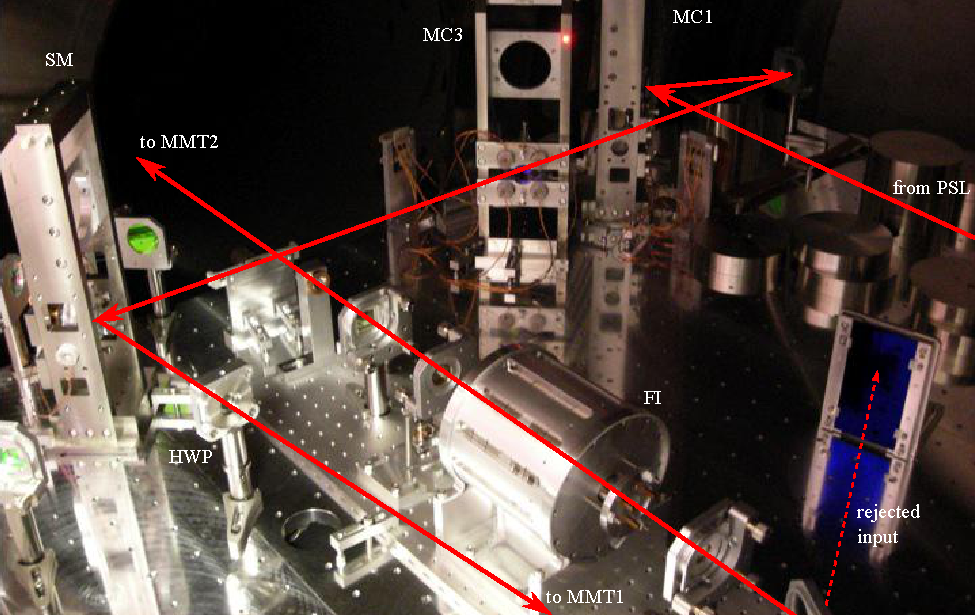
\includegraphics[width=1.0\textwidth]{figures/HAM1_view1.pdf}}
\subfigure{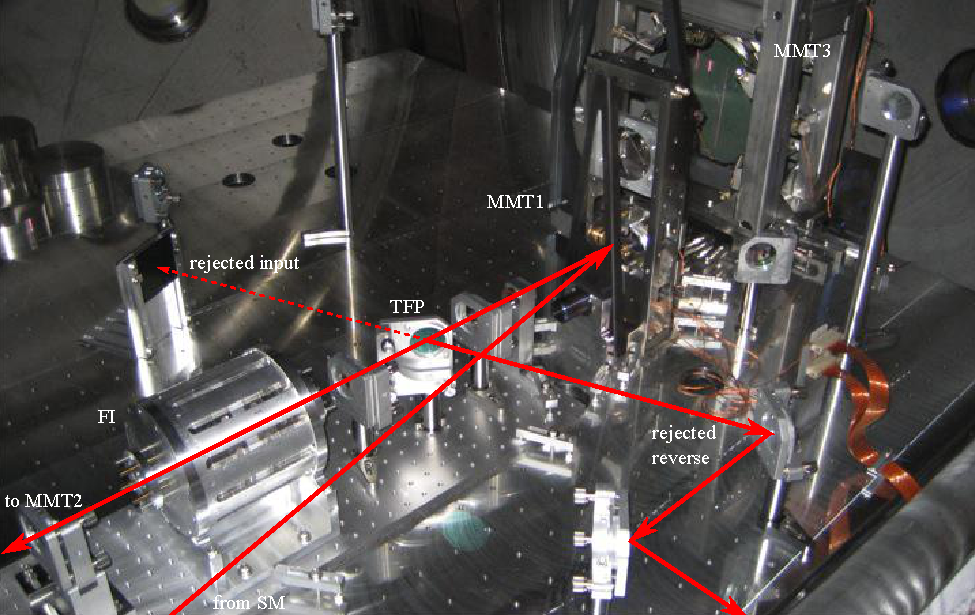
\includegraphics[width=1.0\textwidth]{figures/HAM1_view2.pdf}}
\caption[Photographs of the Enhanced LIGO HAM1 Input Optics \emph{in
  situ}]{Photographs of the Enhanced LIGO HAM1 Input Optics \emph{in
    situ} with a drawing of the beam path superimposed. Photographs
  courtesy of Katherine Dooley.}
\label{fig:IOpictures}
\end{centering}
\end{figure}


\subsection{Electro-optic Modulator Design}
We replaced the commercially-made New Focus 4003 resonant phase
modulator of Initial LIGO with an in-house EOM design and
construction. Both a new crystal choice and architectural design
change allow for superior performance.

The Enhanced LIGO EOM design uses a crystal of rubidium titanyl
phosphate (RTP), which has at most 1/10 the absorption coefficient at
1064 nm of the lithium niobate (LiNbO$_3$) crystal from Initial
LIGO. At 200~W the RTP should produce a thermal lens of 200 m and
higher order mode content of less than 1\%, compared to the 3.3~m lens
the LiNbO$_3$ produces at 10~W. The RTP has a minimal risk of damage,
since it has both twice the damage threshold of LiNbO$_3$ and is
subjected to a beam twice the size of that in Initial LIGO. RTP and
LiNbO$_3$ have similar electro-optic coefficients. Also, RTP's $dn/dT$
anisotropy is 50\% smaller. Table \ref{tab:EOMcrystals} compares the
properties of most interest of the two crystals.

\begin{table}
\centering
\caption[Comparison of selected properties of the Initial and Enhanced
LIGO EOM crystals]{Comparison of selected properties of the Initial and Enhanced
  LIGO EOM crystals, LiNbO$_3$ and RTP, respectively. RTP was
  preferred for Enhanced LIGO because of its lower absorption,
  superior thermal properties, and similar 
  electro-optic properties \citep{UFLIGOGroup2006Upgrading}.}  
\begin{tabular}{l l r@{}l r@{}l}
\hline
 & units & \multicolumn{2}{l}{LiNbO$_3$} & \multicolumn{2}{l}{RTP} \\
\hline
damage threshold & MW/cm$^2$ & 280 & & $>$600 & \\
absorption coeff. at 1064 nm & ppm/cm & $<$5000 & & $<$500 & \\
electro-optic coeff. ($n_z^3 r_{33}$) & pm/V & 306 & & 239 & \\
$dn_y/dT$ & 10$^{-6}$/K & 5 & .4 & 2 & .79 \\
$dn_z/dT$ & 10$^{-6}$/K & 37 & .9 & 9 & .24 \\
\hline
\end{tabular}
\label{tab:EOMcrystals}
\end{table}

We procured the RTP crystals from Raicol and packaged them into
specially-designed, custom-built modulators. The crystal dimensions are
$4 \times 4 \times 40$ mm and their faces are wedged by $2.85^\circ$
and anti-reflection (AR) coated. The wedge serves to separate the
polarizations and prevents an etalon effect, resulting in a
suppression of amplitude modulation. Only one crystal is used in the
EOM in order to reduce the number of surface reflections. Three
separate pairs of electrodes, each with its own resonant LC circuit,
are placed across the crystal in series, producing the three required
sets of RF sidebands: 24.5~MHz, 33.3~MHZ and 61.2~MHz. A diagram is
shown in Figure \ref{fig:EOM}. Reference
\citep{Quetschke2008ElectroOptic} contains further details about the
modulator architecture.

\begin{figure}
\begin{centering}
  \subfigure[]{\includegraphics{figures/EOMthesis.pdf}}
  \subfigure[]{\includegraphics{figures/EOMcircuit_thesis.pdf}}
  \caption[Electro-optic modulator design]{Electro-optic modulator
    design. A) The single RTP crystal is sandwiched between three sets
    of electrodes that apply three different modulation
    frequencies. The wedged ends of the crystal separate the
    polarizations of the light. The p-polarized light is used in the
    interferometer. B) A schematic for each of the three impedance
    matching circuits of the EOM. For the three sets of electrodes,
    each of which creates its own $C_{crystal}$, a capacitor is placed
    parallel to the LC circuit formed by the crystal and a hand-wound
    inductor.  The circuits provide 50~$\Omega$ input impedance on
    resonance and are housed in a separate box from the crystal.}
\label{fig:EOM}
\end{centering}
\end{figure}

\subsection{Mode Cleaner Design}
The mode cleaner is a suspended 12.2~m long triangular ring cavity
with finesse $\mathcal{F}$=1280 (refer to Appendix~\ref{sec:MCpole}
for a measurement of the finesse) and free spectral range of
12.243~MHz. The three mirror architecture was selected over the
standard two mirror linear filter cavity because it acts as a
polarization filter and because it eliminates direct path back
propagation to the laser \citep{Raab1992Estimation}.  A pick-off of the
reflected beam is naturally facilitated for use in generating control
signals. A potential downside to the three mirror design is the
introduction of astigmatism, but this effect is negligible due to the
small opening angle of the MC. 

The MC has a round-trip length of 24.5~m. The beam waist has a radius of
1.63~mm and is located between the two 45$^\circ$ flat mirrors, MC1 and
MC3. See Figure \ref{fig:IOschematic}). A concave third mirror, MC2,
18.15~m in radius of curvature, forms the far point of the mode
cleaner's isosceles triangle shape. The power stored in the MC is 408
times the amount coupled in, equivalent to about 2.7~kW in Initial
LIGO and at most 11~kW for Enhanced LIGO. The peak irradiances are
32~kW/cm$^2$ and 132~kW/cm$^2$ for Initial LIGO and Enhanced LIGO,
respectively.

The mode cleaner mirrors are 75 mm in diameter and 25 mm thick. The
substrate material is fused silica and the mirror coating is made of
alternating layers of silica and tantala. In order to reduce the
absorption of heat in these materials and therefore improve the
transmission and modal quality of the beam in the mode cleaner, we
removed particulate by drag wiping the surface of the MC mirrors with
methanol and optical tissues. The mode cleaner was otherwise identical
to that in Initial LIGO.



\subsection{Faraday Isolator Design}
The Enhanced LIGO Faraday isolator design required not only the use of
low absorption optics, but additional design choices to mitigate any
residual thermal lensing and birefringence. In addition, trade-offs
between optical efficiency in the forward direction, optical isolation
in the backwards direction, and feasibility of physical access of the
return beam for signal use were considered. The result is that the
Enhanced LIGO Faraday isolator needed a completely new architecture
and new optics compared to both the Initial LIGO FI and commercially
available isolators.

Figure \ref{fig:FI} shows a schematic of the Enhanced LIGO Faraday
Isolator. It begins and ends with low absorption calcite wedge
polarizers (CWP). Between the CWPs is a thin film polarizer (TFP), a
deuterated potassium dihydrogen phosphate (DKDP) element, a half-wave
plate (HWP), and a Faraday rotator. The rotator is made of two low
absorption terbium gallium garnet (TGG) crystals sandwiching a quartz
rotator (QR) inside a 7-disc magnet with a maximum field strength of
1.16~T. The forward propagating beam upon passing through the TGG, QR,
TGG, and HWP elements is rotated by $+22.5^\circ - 67.5^\circ +
22.5^\circ + 22.5^\circ = 0^\circ$. In the reverse direction, the
rotation through HWP, TGG, QR, TGG is $-22.5^\circ + 22.5^\circ +
67.5^\circ + 22.5^\circ = 90^\circ$. The TGG crystals are
non-reciprocal devices while the QR and HWP are reciprocal.

\begin{figure}
\begin{centering}
\subfigure{\includegraphics[width=0.9\columnwidth]{figures/FI_cropped2.jpg}}
\subfigure{\includegraphics{figures/FI_thesis.pdf}}
\caption[Faraday isolator photograph and schematic.]{Faraday isolator
  photograph and schematic. The Faraday isolator preserves the
  polarization of the light in the forward-going direction and rotates
  it by 90 degrees in the reverse direction. Light from the MC enters
  from the left and exits at the right towards the interferometer. It
  is ideally p-polarized, but any s-polarization contamination is
  promptly diverted $\sim 10$ mrad by the CWP and then reflected by
  the TFP and dumped. The p-polarized reflected beam from the
  interferometer enters from the right and is rotated to s-polarized
  light which is picked-off by the TFP and sent to the Interferometer
  Sensing and Control (ISC) table. Any imperfections in the Faraday
  rotation of the interferometer return beam results in p-polarized
  light traveling backwards along the original input path. Photograph
  courtesy of Katherine Dooley.}
\label{fig:FI}
\end{centering}
\end{figure}

\subsubsection{Thermal birefringence} 
Thermal birefringence is addressed in the Faraday rotator by the use
of the two TGG crystals and one quartz rotator rather than the typical
single TGG \citep{Khazanov2000Suppression}.  In this configuration,
any thermal polarization distortions that the beam experiences while
passing through the first TGG rotator will be mostly undone upon
passing through the second. The multiple elements in the magnet
required a larger magnetic field than in Initial LIGO.
%\textcolor{blue}{(Add sentence of further explanation.)} 
The 7-disc magnet is 130~mm in diameter and 132~mm long and placed in
housing 155~mm in diameter and 161~mm long. The TGG diameter is 20~mm.

\subsubsection{Thermal lensing}  
Thermal lensing in the Faraday isolator is addressed by including
DKDP, a negative $dn/dT$ material, in the beam path. Absorption of
light in the DKDP results in a de-focusing of the beam, which
partially compensates for the thermal focusing induced by absorption
in the TGGs \citep{Mueller2002Method, Khazanov2004Compensation}.  The
optical path length (thickness) of the DKDP is chosen to slightly
over-compensate the positive thermal lens induced in the TGG crystals,
anticipating other positive thermal lenses in the system.

\subsubsection{Polarizers}  
The polarizers used (two CWPs and one TFP) each offer advantages and
disadvantages related to optical efficiency in the forward-propagating
direction, optical isolation in the reflected direction, and thermal
beam drift. The CWPs have very high extinction ratios ($>10^5$) and
high transmission ($>$ 99\%) contributing to good optical efficiency
and isolation performance. However, the angle separating the exiting
orthogonal polarizations of light is very small, on the order of 10
mrad. This small angle requires the light to travel relatively large distances
before we can pick off the beams
needed for interferometer sensing and control. In addition, thermally
induced index of refraction gradients due to the 4.95$^{\circ}$ wedge
angle of the CWPs result in thermal drift. However, the CWPs for the
Enhanced LIGO Faraday have a measured low absorption of 0.0013
cm$^{-1}$
%(from eLIGO wiki) 
with an expected thermal lens of 60~m at 30~W and drift of less than
1.3 $\mu$rad/W \citep{UFLIGOGroup2006Upgrading}.

The advantages of the thin film polarizer over the calcite wedge
polarizer are that it exhibits negligible thermal drift when compared
with CWPs and it operates at the Brewster angle of 55$^\circ$, thus
diverting the return beam in an easily accessible way. However, the
TFP has a lower transmission than the CWP, about 96\%, and an
extinction ratio of only 10$^3$.

Thus, the combination of CWPs and a TFP combines the best of each to
provide a high extinction ratio (from the CWPs) and ease of reflected
beam extraction (from the TFP). The downsides that remain when using
both polarizers are that there is still some thermal drift from the
CWPs. Also the transmission is reduced due to the TFP and to the fact
that there are 16 surfaces from which light can scatter.

\subsubsection{Heat conduction}
\label{sec:heatconduction}
Faraday isolators operating in a vacuum environment suffer from
increased heating with respect to those operating in air. Convective
cooling at the faces of the optical components is no longer an
effective heat removal channel, so proper heat sinking is essential to
minimize thermal lensing and depolarization. It has been shown that
Faraday isolators carefully aligned in air can experience a dramatic
reduction in isolation ratio ($>$ 10-15 dB) when placed in vacuum
\citep{TheVIRGOCollaboration2008Invacuum}. The dominant cause is the
coupling of the photoelastic effect to the temperature gradient
induced by laser beam absorption. Also of importance is the
temperature dependence of the Verdet constant--different spatial parts
of the beam experience different linear polarization rotations in the presence
of a temperature gradient \cite{Barnes1992Variation}.

\begin{figure}
\begin{centering}
\includegraphics{figures/TGG_scaled.jpg}
\caption[Photograph of an indium-wrapped TGG crystal]{Photograph of TGG crystal
  with indium foil wrapping. Photograph courtesy of Katherine Dooley.}
\label{fig:TGG}
\end{centering}
\end{figure}

To improve heat conduction away from the Faraday rotator optical
components, we designed housing for the TGG and quartz crystals that
provided improved heat sinking to the Faraday rotator. We also wrapped
the TGGs with indium foil as pictured in Figure \ref{fig:TGG} to improve
contact with the housing, and we cushioned the DKDP and the HWP with
indium wire in their aluminum holders. This has the additional effect
of avoiding the development of thermal stresses in the crystals, an
especially important consideration for the very fragile DKDP.


\subsection{Mode-matching Telescope Design}
% from May 31, 2007 elog
The mode matching into the interferometer (at Livingston) was measured
to be at best 90\% in Initial LIGO. Because of the stringent
requirements placed on the LIGO vacuum system to reduce phase noise
through scattering by residual gas, standard opto-mechanical
translators are not permitted in the vacuum; it is therefore not
possible to physically move the mode matching telescope mirrors while
operating the interferometer. Through a combination of needing to move
the MMTs in order to fit the new Faraday isolator on the in-vacuum
optics table and additional measurements and models to determine how
to improve the coupling, a new set of MMT positions was chosen for
Enhanced LIGO. Fundamental design considerations are discussed in
Ref. \citep{Delker1997Design}.



\section{Performance of the Enhanced LIGO Input Optics}
\label{sec:performance}
The most convincing figure of merit for the Input Optics performance
is that the Enhanced LIGO interferometers achieved low-noise operation
with 20 W input power without thermal issues from the
IO. Additionally, the Input Optics were operated successfully up to
the available 30 W of power.  (Instabilities with other interferometer
subsystems limited the Enhanced LIGO science run operation to 20~W.)
We present in this section detailed measurements of the Input Optics
performance during Enhanced LIGO. Specific measurements and results
presented in figures and the text come from Livingston; performance at
Hanford was similar and is included in tables summarizing the results.



\subsection{Optical Efficiency}
The optical efficiency of the Enhanced LIGO Input Optics from EOM to
recycling mirror was 75\%, a marked improvement over the approximate
60\% that was measured for Initial LIGO. A substantial part of the
improvement came from the discovery and subsequent correction of a
6.5\% loss at the second of the in-vacuum steering mirrors directing
light into the MC (refer to Figure \ref{fig:IOschematic}). A 45$^\circ$
reflecting mirror had been used for a beam with an 8$^\circ$ angle of
incidence. Losses attributable to the mode cleaner and Faraday
isolator are described in the following sections. A summary of the IO
power budget is found in Table \ref{tab:pwrbudget}.

\begin{table}
\centering
\caption[Enhanced LIGO Input Optics power budget.]{Enhanced LIGO Input
  Optics power budget. Errors are $\pm 1\%$, except for the TFP loss
  whose error is $\pm 0.1\%$. The 
  composite mode cleaner transmission is the percentage of power after the MC to
  before the MC and is the product of the MC visibility and
  transmission. Initial LIGO values,
  where known, are included in parentheses and have errors of several percent.}
\begin{tabular}{l r@{}l r@{}l}
\hline
 & \multicolumn{2}{l}{Livingston} & \multicolumn{2}{l}{Hanford} \\
\hline
Mode cleaner visibility & 92 & \% & 97 & \% \\
Mode cleaner transmission & 88 & \% & 90 & \% \\
Composite MC transmission & 81 & \% (72\%) & 87 & \% \\
Faraday transmission &       93 & \% (86\%) & 94 & \% (86\%) \\
\hspace{0.5cm} - Thin film polarizer loss & 4 & .0\% & 2 & .7\% \\ 
IO efficiency (PSL to RM) & 75 & \% (60\%) & 82 & \% \\
\hline
\end{tabular}
\label{tab:pwrbudget}
\end{table}


\subsubsection{Mode cleaner losses} 
The mode cleaner was the greatest single source of power loss in both
Initial and Enhanced LIGO. The mode cleaner visibility, defined here as
\begin{equation}
\mbox{visibility} = \frac{P_{\mathrm{in}} - P_{\mathrm{reflected}}}{P_{\mathrm{in}}},
\end{equation}
the ratio of the amount of light coupled into the MC to the amount
impinging the MC input mirror, was 92\%. Visibility
reduction is the result of higher order mode content of $P_{\mathrm{in}}$
and mode mismatch into the MC. The visibility was constant within
0.04\% up to 30~W input power at both sites, providing a positive
indication that thermal aberrations in the MC and upstream
were negligible.

Of the light coupled into the MC, 88\% was transmitted,
corresponding to an average loss of 98 ppm per mirror.  The scatter
loss, $[4 \pi \sigma_{rms} / \lambda]^2$, is expected to be 22
ppm/mirror based on the mirrors' measured root mean square surface
microroughness of $\sigma_{rms}< 0.4$ nm \cite{1998Component}. Part of
the discrepancy between expectation and measurement was determined to
come from poor or damaged AR coatings. We measured a 1.3\% reflection
from the AR coatings on MC mirrors at both Livingston and Hanford, a
transmitted power loss equivalent to 10~ppm of intracavity loss per
mirror.

\begin{figure}
\begin{centering}
\includegraphics[width=1.0\columnwidth]{figures/MCdrumheadFeb08_cropped.png}
\caption[Data from the mode cleaner absorption measurement]{Data from
  the mode cleaner absorption measurement. 
%\footnote{Credit: Valera Frolov} 
  Power into the MC was cycled between 0.9~W and 5.1~W at 3 hour
  intervals (bottom frame) and the change in frequency of the drumhead
  mode of each mirror was recorded (top frame). The ambient
  temperature (middle frame) was also recorded in order to correct for
  its effects.}
%\textcolor{blue}{This is Valera's plot from Feb. 9, 2008}
\label{fig:MCabsorption}
\end{centering}
\end{figure}

\begin{table}
\centering
\caption[Absorption values for the Livingston and Hanford mode
cleaner mirrors]{Absorption values for the Livingston and Hanford mode
  cleaner mirrors before (in parentheses) and after drag wiping. The precision is $\pm 10\%$.} 
%(from the March 8, 2008 elog and uses Muzammil's factor of $14/48$ correction.)
\begin{tabular}{l r@{.}l r@{.}l}
\hline
mirror & \multicolumn{2}{l}{Livingston} & \multicolumn{2}{l}{Hanford}\\
% mirror & before & after & before & after \\
% \hline\hline
% MC1 & 18.7 & 2.1  & 6.1  & 5.8 \\
% MC2 & 5.5  & 2.0  & 23.9 & 7.6 \\
% MC3 & 12.8 & 3.4  & 12.5 & 15.6 \\
\hline
MC1 & 2&1 ppm (18.7 ppm) & 5&8 (6.1 ppm) \\
MC2 & 2&0 ppm (5.5 ppm) & 7&6 (23.9 ppm) \\
MC3 & 3&4 ppm (12.8 ppm) & 15&6 (12.5 ppm) \\
\hline
\end{tabular}
\label{tab:MCabsorption2}
\end{table}

Another source of MC losses is via absorption of heat by particulates
residing on the mirror's surface. We measured the absorption with a
technique that makes use of the frequency shift of the thermally
driven drumhead eigenfrequencies of the mirror substrate
\citep{Punturo2007Mirror}. The frequency shift directly correlates
with the MC absorption via the substrate's change in Young's modulus
with temperature, $dY/dT$. A finite element model (COMSOL
\cite{COMSOL}) was used to compute the expected frequency shift from a
temperature change of the substrate resulting from the mirror coating
absorption. The measured eigenfrequencies for each mirror at room
temperature are 28164~Hz, 28209~Hz, and 28237~Hz, respectively.

We cycled the power into the mode cleaner between 0.9~W and 5.1~W at 3
hour intervals, allowing enough time for a thermal characteristic time
constant to be reached.  At the same time, we recorded the frequencies
of the high Q drumhead mode peaks as found in the mode cleaner
frequency error signal, heterodyned down by 28~kHz. Figure
\ref{fig:MCabsorption} shows the measurement data. Correcting for
ambient temperature fluctuations, we find a frequency shift of 0.043,
0.043, and 0.072 Hz/W. As a result of drag-wiping the mirrors, the
absorption decreased for all but one mirror, as shown for both Hanford
and Livingston in Table~\ref{tab:MCabsorption2}.


\subsubsection{Faraday isolator losses} 
The Faraday isolator was the second greatest source of power loss with
its transmission of 93\%. This was an improvement over the
86\% transmission of the Initial LIGO FI. The most lossy element in the
Faraday isolator was the thin film polarizer, accounting for 4\% of
total losses. The integrated losses from AR coatings and absorption in the
TGGs, CWPs, HWP, and DKDP account for the remaining 3\% of missing power. 


\subsection{Faraday Isolation Ratio}
The isolation ratio is defined as the ratio of power incident on the
Faraday in the reverse direction (the light reflected from the
interferometer) to the power transmitted in the 
reverse direction and is often quoted in decibels: isolation ratio~=~$10
\log_{10}(P_{in-reverse}/P_{out-reverse})$.  We measured the isolation ratio of the
Faraday isolator as a function of input power both in air prior to
installation and \emph{in situ} during Enhanced LIGO operation.

To measure the in-vacuum isolation ratio, we misaligned the
interferometer arms so that the input beam would be 
promptly reflected off of the $97\%$ reflective recycling mirror. This
also has the consequence that 
the Faraday isolator is subjected to twice the input
power. Our isolation monitor was a pick-off of the backwards 
transmitted beam taken immediately after transmission
through the Faraday that we sent out of a vacuum chamber
viewport. Refer to the ``isolation check beam'' in 
Figure~\ref{fig:IOschematic}. The in air measurement was done similarly,
except in an optics lab with a reflecting mirror placed directly after
the Faraday. 

\begin{figure}
\begin{centering}
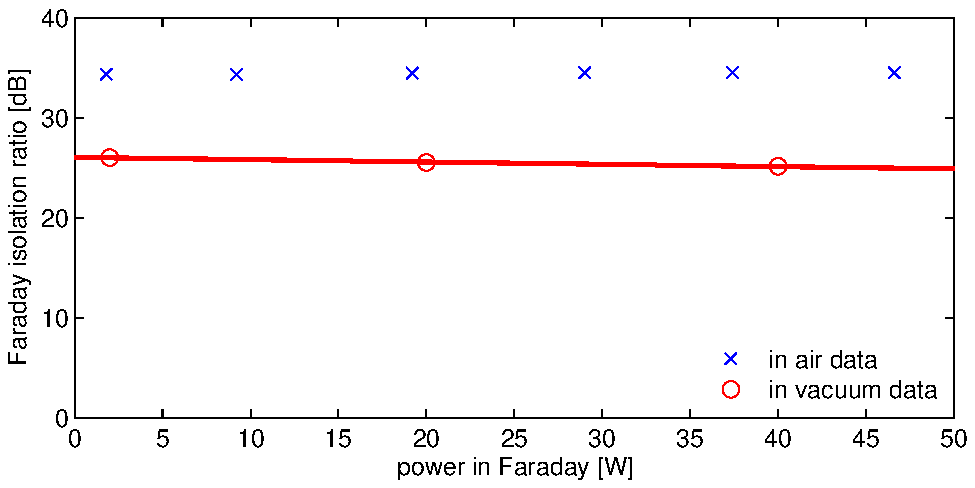
\includegraphics[width=1.0\columnwidth]{figures/FaradayIR.pdf}
\caption[Faraday isolator isolation ratio as measured in air and in
vacuum]{Faraday isolator isolation ratio as measured in air prior to
  installation and \emph{in situ} in vacuum. The isolation worsens by
  a factor of 6 upon placement of the Faraday in vacuum. The linear
  fits to the data show a constant in-air isolation ratio and an
  in-vacuum isolation ratio degradation of 0.02 dB/W.}
\label{fig:IR}
\end{centering}
\end{figure}

Figure \ref{fig:IR} shows our isolation ratio data. Most notably, we
observe an isolation decrease of a factor of six upon placing the
Faraday isolator in vacuum, a result consistent with that reported by
Ref. \citep{TheVIRGOCollaboration2008Invacuum}. In air the isolation
ratio is a constant 34.46 $\pm$ 0.04 dB from low power up to 47~W, and
in vacuum the isolation ratio is 26.5 dB at low power. The underlying
cause is the absence of cooling by air convection. If we attribute the
loss to the TGGs, then based on the change in TGG polarization
rotation angle necessary to produce the measured isolation drop of
8~dB and the temperature dependence of the TGG's Verdet constant, we
can put an upper limit of 11~K on the crystal temperature rise from
air to vacuum. Furthermore, a degradation of 0.02~dB/W is measured in
vacuum.

\subsection{Thermal Steering}
We measured the \emph{in situ} thermal angular drift of both the beam
transmitted through the mode cleaner and of the reflected beam from
the Faraday isolator with up to 25~W input power. Just as for the
isolation ratio measurement, we misaligned the interferometer arms so
that the input beam would be promptly reflected off of the recycling
mirror. The Faraday rotator was thus subjected to up to 50~W total
and the MC to 25~W. 

Pitch and yaw motion of the mode cleaner transmitted and
interferometer reflected beams were recorded using the quadrant
photodiode (QPD) on the Input Optics table and the RF alignment
detectors on the Interferometer Sensing and Control table, as seen in
Figure~\ref{fig:IOschematic}. There are no lenses between the MC waist
and its measurement QPD, so only the path length between the two were
needed to calibrate in radians the pitch and yaw signals on the
QPD. The interferometer reflected beam, however, passes through
several lenses. Thus, ray transfer matrices and the two alignment
detectors were necessary to extract the Faraday drift
calibration. Details of the calibration method are presented in
Appendix~\ref{sec:driftcal}.

Figure \ref{fig:drift} shows the calibrated beam steering data. The
angle of the beam out of the mode cleaner does not change measurably
as a function of input power in yaw (4.7~nrad/W) and changes by only
440~nrad/W in pitch. For the Faraday isolator, we record a beam drift
originating at the center of the Faraday rotator of 1.8~\microrad/W in
yaw and 3.2~\microrad/W in pitch. Therefore, when ramping the input
power up to 30~W during a full interferometer lock, the upper limit on
the drift experienced by the reflected beam is about 100
\microrad. This is a thirty-fold reduction with respect to the Initial
LIGO Faraday isolator and represents a fifth of the beam's divergence
angle, $\theta_{div}$~=~490 \microrad.

\begin{figure}
\begin{centering}
% \includegraphics[width=1.0\columnwidth]{figures/MC_FI_drift_labelled.pdf}
\subfigure[]{\includegraphics[width=1.0\columnwidth]{figures/forthesis_refldriftx10.pdf}}
\subfigure[]{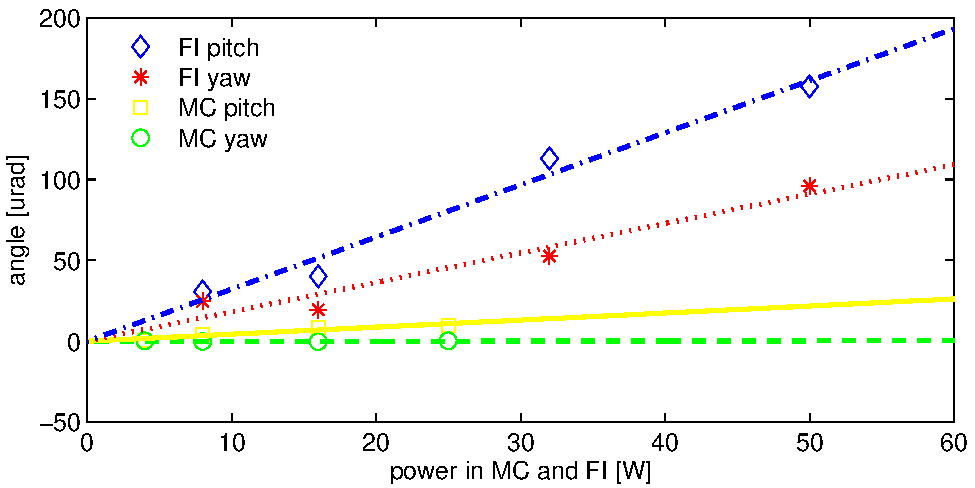
\includegraphics[width=1.0\columnwidth]{figures/alldrift.pdf}}
\caption[Mode cleaner and Faraday isolator thermal drift data.]{Mode
  cleaner and Faraday isolator thermal drift data. A) Angular motion
  of the beam at the MC waist and FI rotator as the input power is
  stepped. The beam is double-passed through the Faraday isolator, so
  it experiences twice the input power. B) Average beam angle per
  power level in the MC and FI. Linear fits to the data are also
  shown. The slopes for MC yaw, MC pitch, FI yaw, and FI pitch,
  respectively, are 0.0047, 0.44, 1.8, and 3.2 \microrad/W.}
\label{fig:drift}
\end{centering}
\end{figure}


\subsection{Thermal Lensing}
We measured the profiles of both the beam transmitted through the
mode cleaner and the reflected beam picked off by the Faraday isolator
at low ($\sim$~1~W) and high ($\sim$~25~W) input powers to assess the
degree of thermal lensing induced in the MC and FI. Again, we
misaligned the interferometer arms so that the input beam would be
promptly reflected off the recycling mirror. We picked off a fraction
of the reflected beam on the Interferometer Sensing and Control table
and of the mode cleaner transmitted beam on the Input Optics table
(refer to Figure \ref{fig:IOschematic}), placed lenses in each of their
paths, and measured the beam diameters at several locations on either
side of the waists created by the lenses. A change in the beam waist
size or position as a function of laser power indicates the presence
of a thermal lens.

\begin{figure}
\begin{centering}
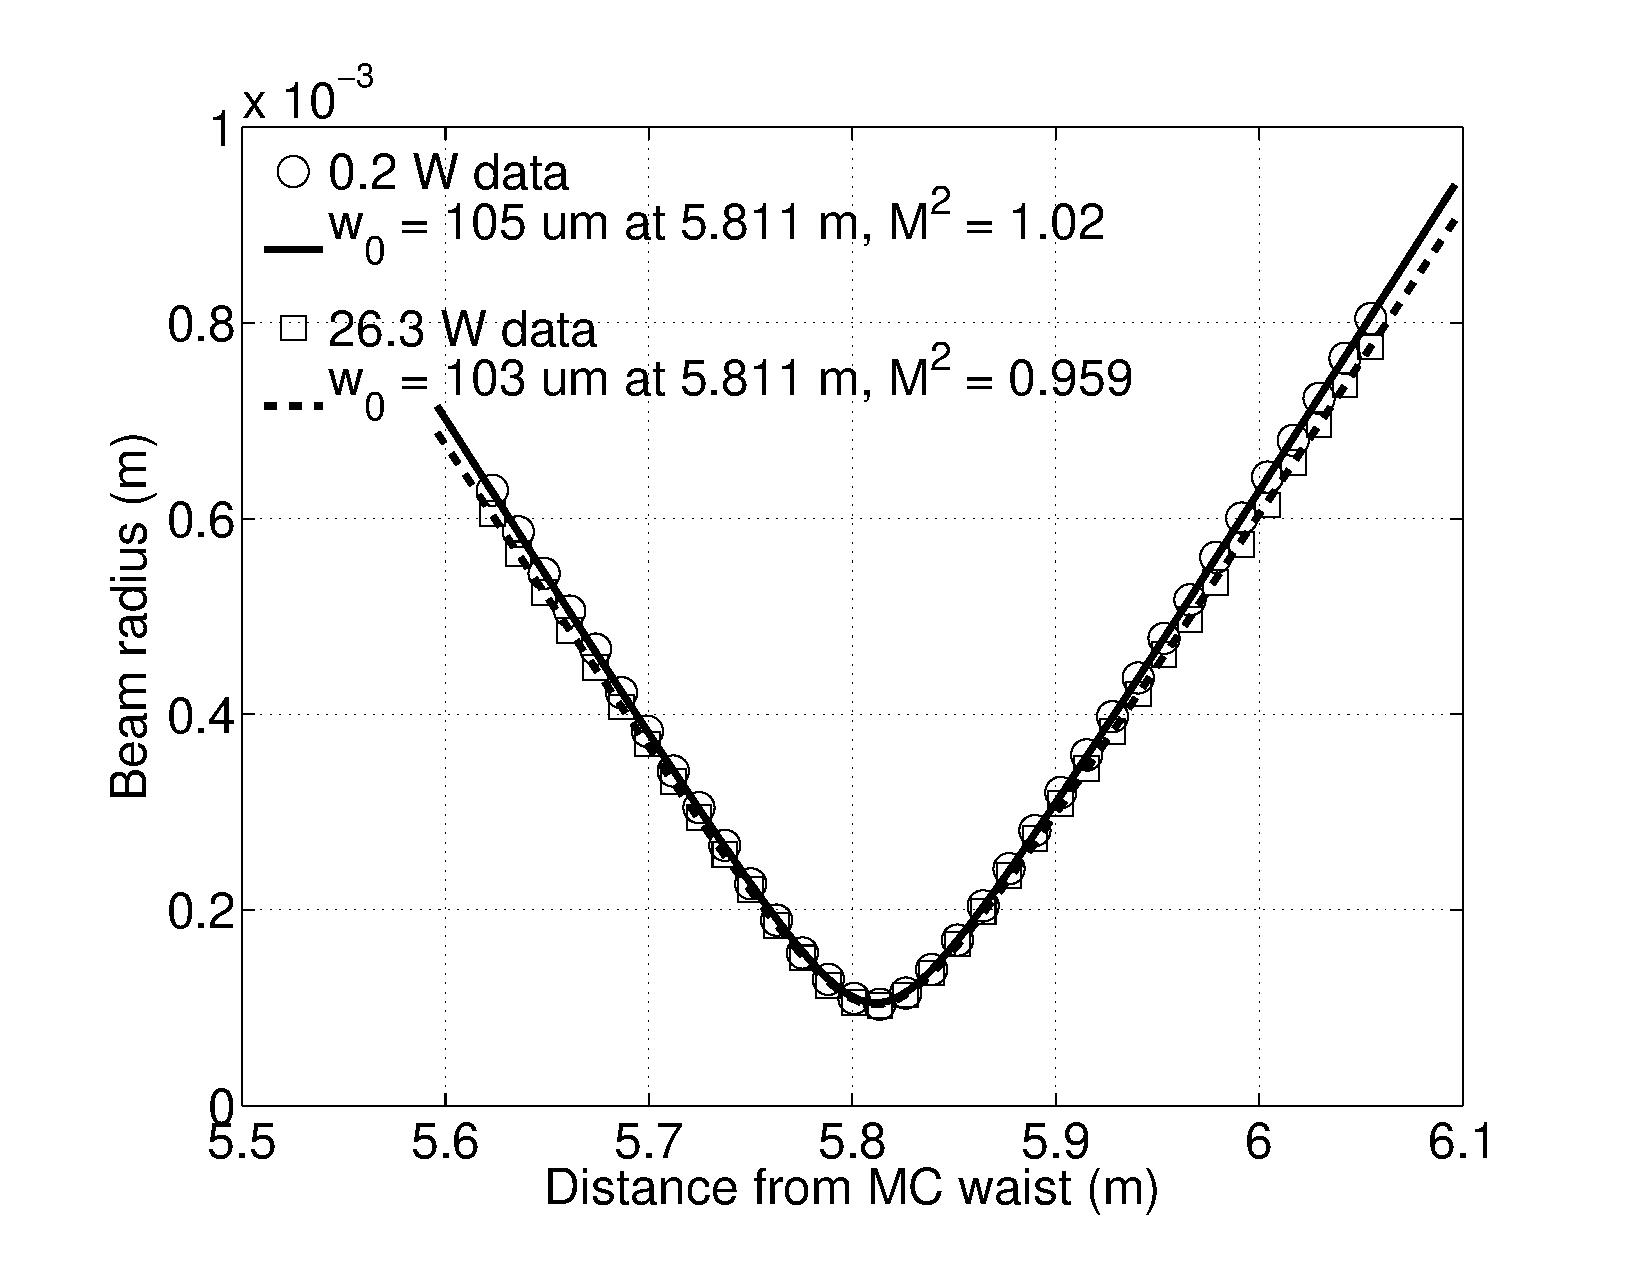
\includegraphics[width=1.0\columnwidth]{figures/MCTrans_datafit.pdf}
\caption[Profile at high and low powers of mode cleaner transmitted
beam]{Profile at high and low powers of a pick-off of the beam
  transmitted through the mode cleaner. The precision of the beam
  profiler is $\pm 5\%$. Within the error of the measurement, there
  are no obvious degradations.}
\label{fig:MC_lensing}
\end{centering}
\end{figure}

\begin{figure}
\begin{centering}
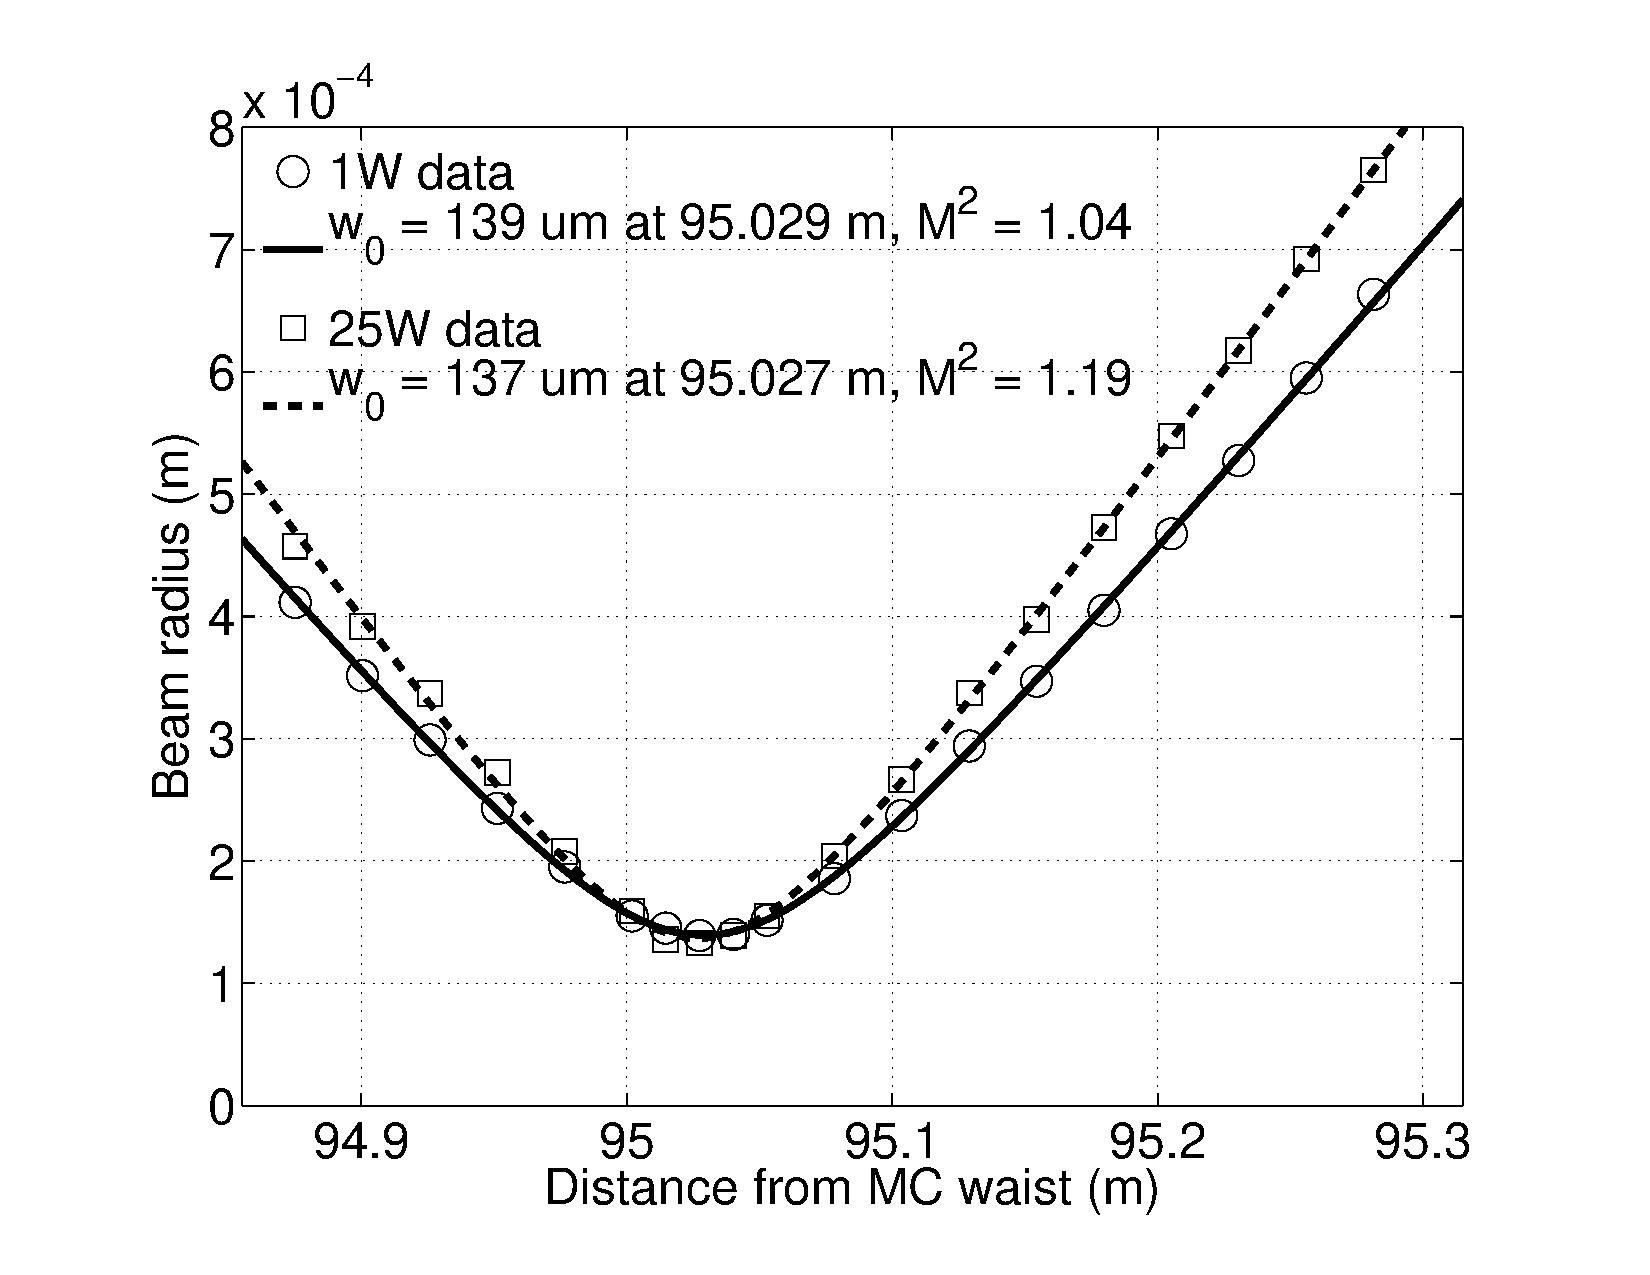
\includegraphics[width=1.0\columnwidth]{figures/REFL_datafit.pdf}
\caption[Faraday isolator thermal lensing data]{Faraday isolator
  thermal lensing data. With 25 W into the Faraday isolator
  (corresponding to 50 W in double pass), the beam has a steeper
  divergence than a pure TEM$_{00}$ beam, indicating the presence of
  higher order modes. Errors are $\pm 5.0\%$ for each data point.}
\label{fig:FI_lensing}
\end{centering}
\end{figure}

As seen in Figure~\ref{fig:MC_lensing} and Figure~\ref{fig:FI_lensing}, the
waists of the two sets of data are collocated: no thermal lens is
measured. For the Faraday isolator, the divergence of the low and high
power beams differs, indicating that the beam quality degrades with
power. The $M^2$ factor at 1~W is 1.04 indicating the beam is 
nearly perfectly a TEM$_{00}$ mode. At 25~W, $M^2$ increases to 1.19,
corresponding to increased higher-order-mode content. The percentage
of power in higher-order modes depends strongly on the mode order and
relative phases of the modes, and thus cannot be determined from this
measurement \citep{Kwee2007Laser}.

The results for the mode cleaner data are consistent with no thermal
lensing. The high and low power beam profiles are within each
other's error bars and well below our requirements. 


\subsection{Mode-matching}
We measured the effectiveness of the mode-matching telescope by taking
the ratio of power at the reflected port when all of the
interferometer cavities are on resonance to the power in the reflected
beam when the cavities are unlocked. Since the impedance matching is
near perfect, all light at the reflected port during interferometer
lock is attributable to a mode mismatch. Initially, anywhere between
10\% and 17\% of the light was rejected by the cavity due to poor,
power-dependent mode matching.  After translating the mode-matching
telescope mirrors during a vacuum chamber incursion and upgrading the
other IO components, the ratio we measured was 8\% independent of
input power. The MMT succeeds at coupling 92\% of the light into the
interferometer at all times, marking both an improvement in MMT mirror
placement and success in eliminating measurable thermal
issues. Appendix~\ref{sec:MM} presents details of the mode-matching
measurement.


\section{Implications for Advanced LIGO}
\label{sec:aLIGO}
As with other Advanced LIGO interferometer components, Enhanced LIGO
served as a technology demonstrator for the Advanced LIGO Input
Optics, albeit at lower laser powers than will be used there. The
performance of the Enhanced LIGO Input Optics components, at 20~W of
input power allows us to infer their performance in Advanced LIGO.
The requirements for the Advanced LIGO Input Optics demand are for
similar performance to Enhanced LIGO, but with almost 8 times the
laser power.

The Enhanced LIGO electro-optic modulator showed no thermal lensing,
degraded transmission, nor damage in over 1 million hours of sustained
operation at 30~W of laser power. Measurements of the thermal lensing
in RTP at powers up to 160 W show a relative power loss of $< 0.4\%$,
indicating that thermal lensing should be negligible in Advanced LIGO.
Peak irradiances in the EOM will be approximately four times that of
Enhanced LIGO (a 45\% larger beam diameter will somewhat offset the
increased power).  Testing of RTP at 10 times the expected Advanced
LIGO irradiance over 100~hours show no signs of damage or degraded
transmission.

The mode cleaner showed no measurable change in operational state as a
function of input power.  This bodes well for the Advanced LIGO mode
cleaner.  Compared with the Enhanced LIGO mode cleaner, the Advanced
LIGO mode cleaner is designed with a lower finesse (520) than Initial
LIGO (1280).  For 150~W input power, the Advanced LIGO mode cleaner
will operate with 3 times greater stored power than Initial LIGO.  The
corresponding peak irradiance is 400~kW/m$^2$, well below the
continuous wave coating damage threshold.  Absorption in the Advanced
LIGO mode cleaner mirror optical coatings has been measured at
0.5~ppm, roughly four times less than the best mirror coating
absorption in Enhanced LIGO, so the expected thermal loading due to
coating absorption should be reduced in Advanced LIGO.  The larger
Advanced LIGO mode cleaner mirror substrates and higher input powers
result in a significantly higher contribution to bulk absorption,
roughly 20 times Enhanced LIGO, however the expected thermal lensing
leads to small change ($< 0.5 \%$) in the output mode
\citep{Arain2007Note}.

The Enhanced LIGO data obtained from the FI allows us to make several
predictions about how it will perform in Advanced LIGO.  The measured
isolation ratio decrease of 0.02~dB/W will result in a loss of 3~dB
for a 150~W power level expected for Advanced LIGO relative to its
cold state.  However, the Advanced LIGO FI will employ an \emph{in
  situ} adjustable half wave plate which will allow for a partial
restoration of the isolation ratio. In addition, a new FI scheme to
better compensate for thermal depolarization and thus yield higher
isolation ratios may be implemented
\cite{Snetkov2011Compensation}. The maximum thermally induced angular
steering expected is 480 \micro rad (using a drift rate of
3.2~\microrad/W), approximately equal to the beam divergence
angle. This has some implications for the Advanced LIGO length and
alignment sensing and control system, as the reflected FI beam is used
as a sensing beam. Operation of Advanced LIGO at high powers will
likely require the use of a beam stabilization servo to lock the
position of the reflected beam on the sensing photodiodes.  Although
no measurable thermal lensing was observed (no change in the beam
waist size or position), the measured presence of higher order modes
in the FI at high powers is suggestive of imperfect thermal lens
compensation by the DKDP.  This fault potentially can be reduced by a
careful selection of the thickness of the DKDP to better match the
absorbed power in the TGG crystals.

\section{Summary}
\label{sec:summary}
In summary, we have presented a comprehensive investigation of the
Enhanced LIGO Input Optics, including the function, design, and
performance of the IO.  Several improvements to the design and
implementation of the Enhanced LIGO IO over the Initial LIGO IO have
lead to improved optical efficiency and coupling to the main
interferometer through a substantial reduction in thermo-optical
effects in the major IO optical components, including the
electro-optic modulators, mode cleaner, and Faraday isolator.  The IO
performance in Enhanced LIGO enables us to infer its performance in
Advanced LIGO, and indicates that high power interferometry will be
possible without severe thermal effects.


% \textcolor{blue}{from Guido: summary of the improvements due to the
%   changes in the IO. More power, better shot noise sensitivity,
%   better range, better upper limits, lessons learned for aLIGO
%   (summary like, the details should be in the previous
%   subsections). Make it glorious and complain that other subsystems
%   (TCS) wasn't able to handle the power. Otherwise this becomes very
%   technical and boring.}

% \section{Radiation pressure in MC}
% \textcolor{blue}{Maybe write up April 4, 2009 notebook derivation of
%   radiation pressure length spring in MC. Also, Rana has a noise
%   budget elog entry April 3, 2009.}
